\begin{frame}{Visão geral do software}
    \begin{itemize}
        \item O software desenvolvido apresenta uma GUI contendo um editor baseado em nós.
        \note[item]{
            ``Editores baseados em nós'' descreve o tipo de GUI que apresenta blocos (chamados de ``nós''), com 0 ou mais pinos de entrada e saída, de forma que ligações sejam feitas na intenção de continuamente modificar dados, geralmente ocorrendo da esquerda para a direita.
        }
        \item Os nós representam partes das equações, como parâmetros, populações e expressões.
    \end{itemize}

    \begin{figure}
        \centering
        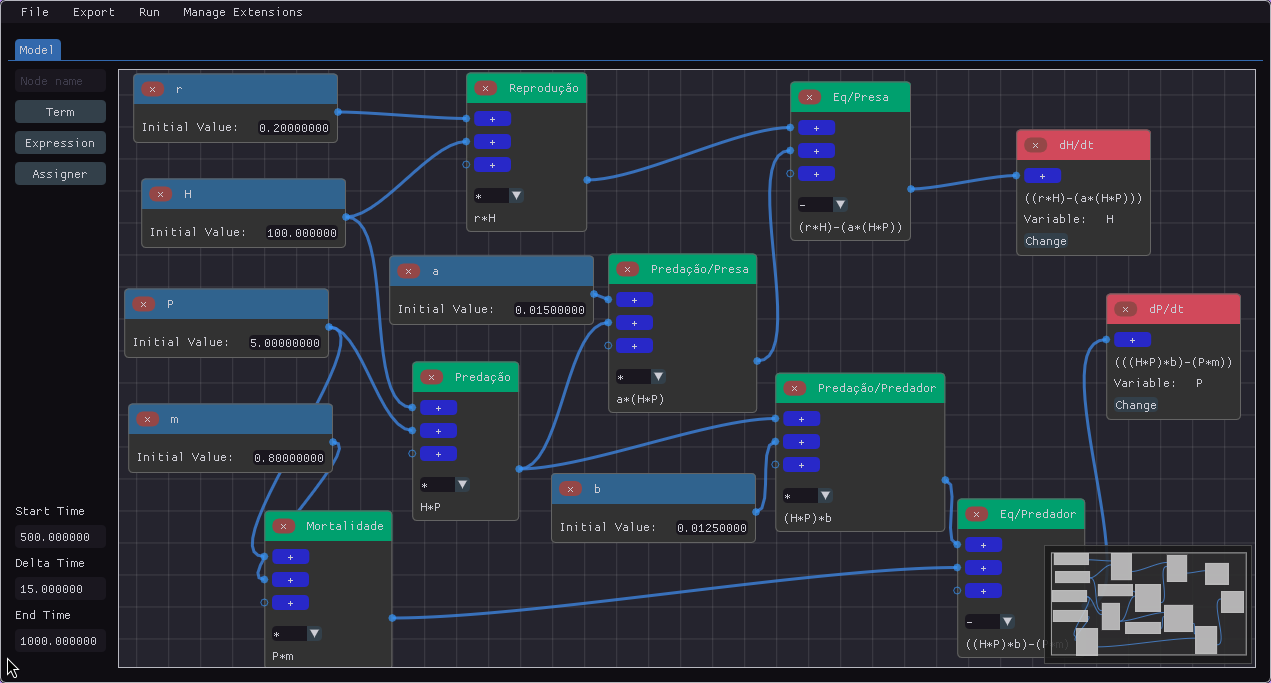
\includegraphics[width=0.75\textwidth]{contents/imgs/ode-designer/predador-presa-fit.png}
    \end{figure}
    \note[item]{Na imagem, podemos ver a representação gráfica do modelo predador-presa.}
\end{frame}

\begin{frame}{Visão geral do software}
    \begin{columns}
        \begin{column}{.5\textwidth}
            Após construído o modelo, o usuário poderá simulá-lo diretamente pela GUI, exportar um PDF dos resultados, ou exportar um código de Python equivalente para o modelo desenhado
            \begin{figure}
                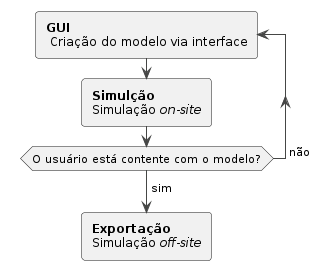
\includegraphics[width=.82\textwidth]{contents/imgs/fluxograma-exp.png}
            \end{figure}
        \end{column}
        \begin{column}{.5\textwidth}
            \begin{figure}
                \centering
                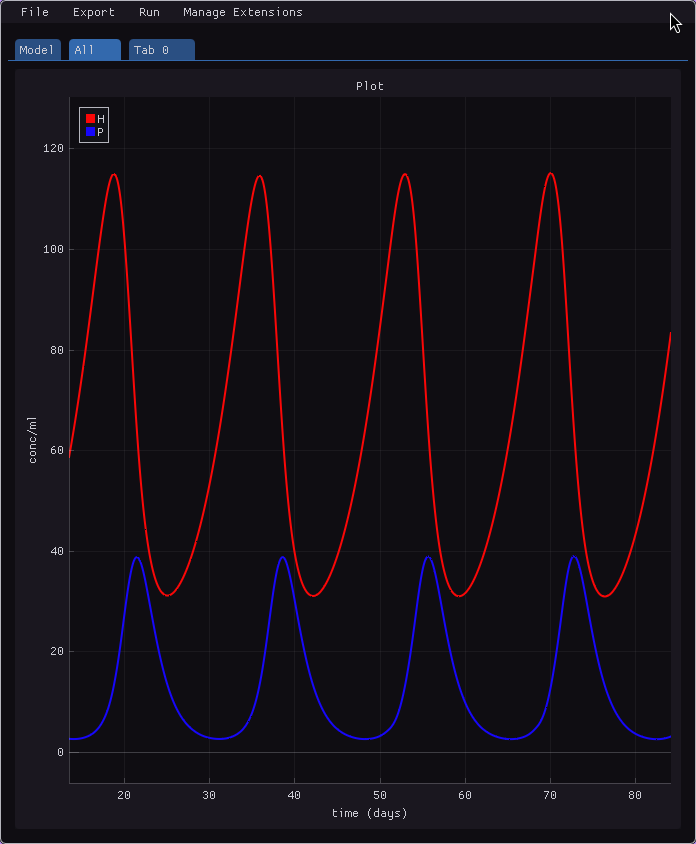
\includegraphics[width=.82\textwidth]{contents/imgs/ode-designer/grafico-thin.png}
            \end{figure}
        \end{column}
    \end{columns}
\end{frame}

\begin{frame}{Representação visual}
    \begin{table}
        \begin{center}
        \begin{tabular}{ m{0.12\textwidth}m{0.5\textwidth}m{0.25\textwidth} }
            \toprule
            Tipo de nó & Usado para representar & Exemplo \\
            \midrule
            Termo & Variáveis, parâmetros e constantes. & $H$, $P$, $a$, $b$, $r$, $m$ \\
            Expressão & Expressões matemáticas que compõem as equações. & \(r.H\), \(a.H.P\), \(r.H - a.H.P\)\\
            Equação & O lado direito de uma EDO. & \(\frac{dH}{dt} = ...\) \\
            \bottomrule
        \end{tabular}
        \end{center}
    \end{table}
    \begin{figure}
        \centering
        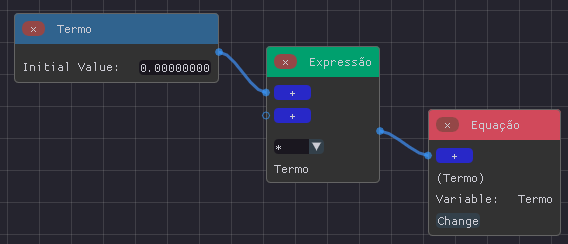
\includegraphics[width=.6\textwidth]{contents/imgs/ode-designer/tipos-nos-slim.png}
    \end{figure}
    \note[item]{
        Estes nós foram projetados para minimizar a dificuldade de uso e a necessidade de manuais. Isso é perceptível pelo fato de que:
        \begin{itemize}
            \item o nó `Termo' possui nenhum pino de entrada e um pino de saída;
            \item O nó `Expressão' possui inúmeros pinos de entrada e um pino de saída;
            \item O nó `Equação' possui um pino de entrada e nenhum pino de saída.
        \end{itemize}
        Deta forma, conclui-se que (1) o nó `Termo' pode ser usado como entrada de `Expressões' e `Equações', (2) o nó `Expressão' pode ser entrada de outras `Expressões' e de `Equações' e (3) o nó `Equação' é terminal.
    }
\end{frame}

\begin{frame}{Árvore de expressões}
    \begin{itemize}
        \item Os nós de Expressão e de Equação carregam consigo árvores de expressões para representar as expressões que constroem.
        \item As árvores são copiadas e enviadas para os nós relacionados quando algum destes eventos ocorrem na interface:
        \begin{itemize}
            \item Mudança de sinal;
            \item Alteração de nome de nós `Termos';
            \item Adições ou remoções de ligações;
            \note[item]{
                Estes eventos podem ocorrer também com subexpressões, que cascateiam as alterações até encontrarem um nó terminal e/ou ainda não ligado a um nó final.
            }
        \end{itemize}
    \end{itemize}
    \begin{figure}
        \centering
        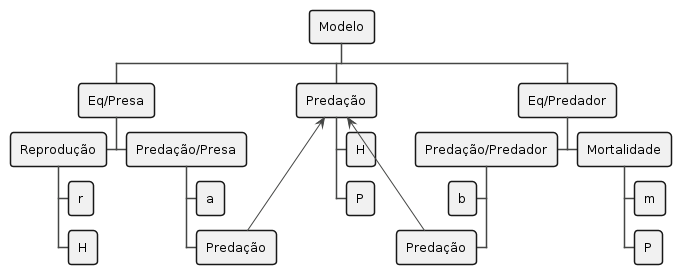
\includegraphics[width=0.7\textwidth]{contents/imgs/expr-tree.png}
    \end{figure}
\end{frame}

\begin{frame}{Representação intermediária}
    \begin{itemize}
        \item Uma representação intermediária foi desenvolvida para simplificar as transformações dos modelos.
        \item A GUI apenas precisa transformar seus modelos na RI. A partir disto, a biblioteca de RI pode gerar códigos em Python e gerar a representação para armazenamento em disco.
        \item A RI foi projetada para ser humanamente legível, possibilitando a recuperação do modelo construído na ausência do software.
    \end{itemize}
\end{frame}

\begin{frame}{Geração de código, simulação interativa e exportação de resultados}
    \begin{itemize}
        \item Os modelos gerados na interface podem ser convertidos para o código em Python equivalente que implementa a simulação.
        \item Este mesmo código também é utilizado pela GUI para gerar os dados necessários para a plotagem dos resultados diretamente na interface.
        \item Similarmente, PDFs podem ser exportados com os mesmos dados.
        \item A utilização das mesmas funções para todas estas exportações e visualizações garante consistência nos resultados obtidos.
    \end{itemize}
\end{frame}

\begin{frame}[fragile]{Geração de código, simulação interativa e exportação de resultados}
    \begin{minted}[fontsize=\footnotesize]{python}
    def initial_values() -> np.ndarray:
        H_0, P_0 = 100.0, 5.0
        return np.array(( H_0, P_0, ))

    def constants() -> list:
        a, b, m, r = 0.015, 0.0125, 0.8, 0.2
        return [ a, b, m, r, ]

    def variable_names() -> list[str]:
        return [ "H", "P", ]

    def system(t: np.float64, y: np.ndarray, *constants) -> np.ndarray:
        H,P, = y
        a,b,m,r, = constants
        dH_dt = (r * H ) - (a * (H * P ) ) 
        dP_dt = ((H * P ) * b ) - (P * m ) 
        return np.array([dH_dt,dP_dt])
    \end{minted}
\end{frame}

\note{
    Destaca-se a legibilidade do código gerado. Para fins apenas de simulação, o código poderia conter variáveis com nomes aleatórios. Contudo, um dos objetivos é exportar este código para facilitar o entendimento do modelo, bem como a sua utilização como ferramenta no ensino-aprendizagem de modelagem computacional.
}

\begin{frame}{Geração de código, simulação interativa e exportação de resultados}
    \begin{figure}
        \centering
        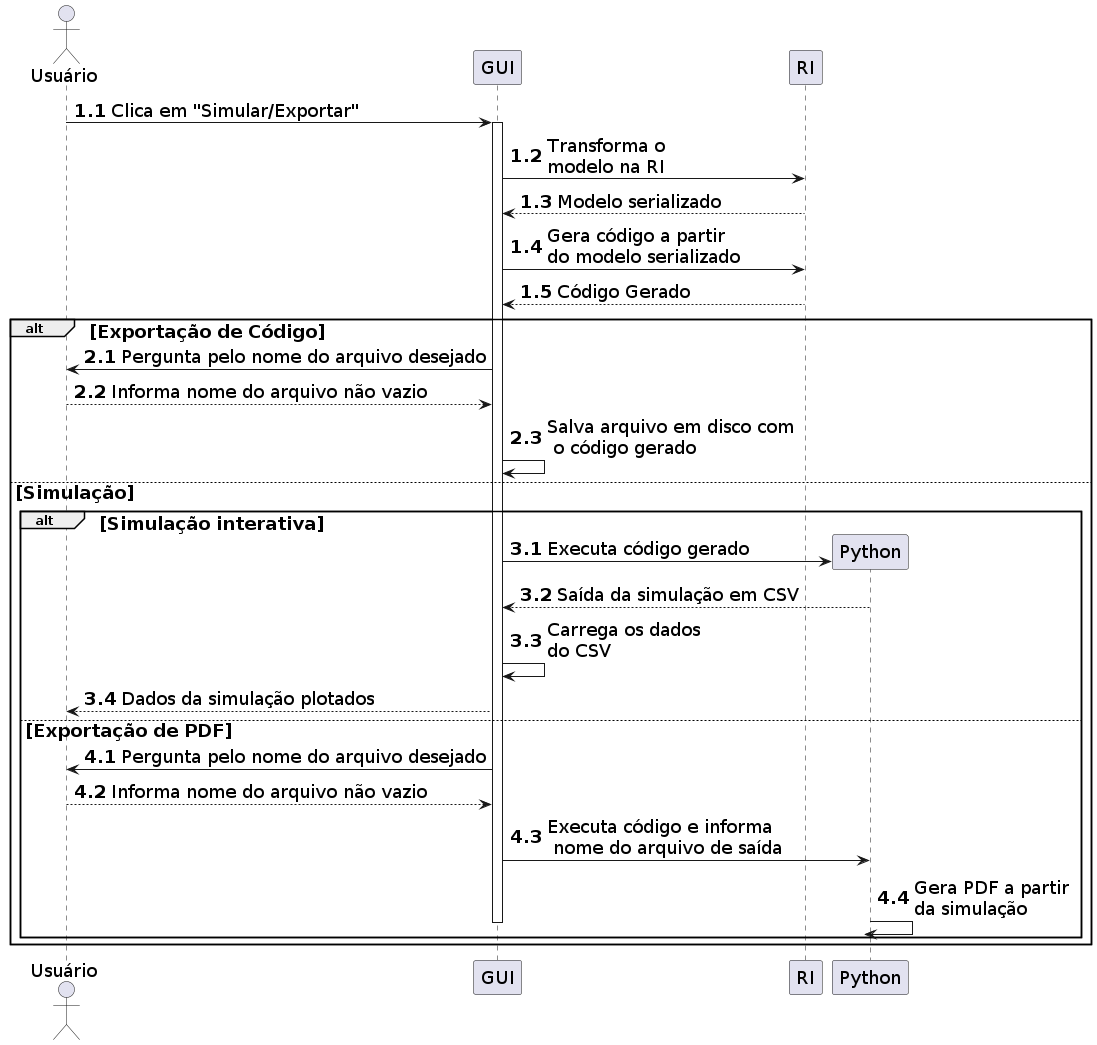
\includegraphics[height=\textheight]{contents/imgs/gui-ri.png}
    \end{figure}
\end{frame}

\begin{frame}[fragile]{Extensibilidade}
    \begin{itemize}
        \item É improvável que apenas as operações básicas sejam o suficiente para construir qualquer sistema de EDOs.
        \item Paralelamente, é impensável construir um software que possui todas as operações matemáticas existentes.
        \item Portanto, uma funcionalidade de extensões foi desenvolvida. O usuário pode utilizar Python para definir nós e as expressões que eles constroem.
        \note[item]{
            Extensões são distribuídas como arquivos de código em Python, que podem ser facilmente compartilhados entre usuários.
        }
        \begin{itemize}
            \item Sendo escrito em Python, o código é apropriado para ser usado nas etapas mencionadas anteriormente, não prejudicando a usabilidade do software.
            \item O software utiliza de trechos de códigos especiais para injetar e inspecionar o código dos usuários a fim de determinar quais funções deveriam representar nós customizados.
        \end{itemize}
    \end{itemize}
\end{frame}

\begin{frame}[fragile]{Extensibilidade}
    \begin{columns}
        \begin{column}{.3\textwidth}
            \begin{minted}{python}
import math

@node
def sin(x):
    return math.sin(x)

@node(format='$1 ^ $2')
def pow(x, y):
    return x ** y
            \end{minted}
        \end{column}
        \begin{column}{.7\textwidth}
            \begin{figure}
                \centering
                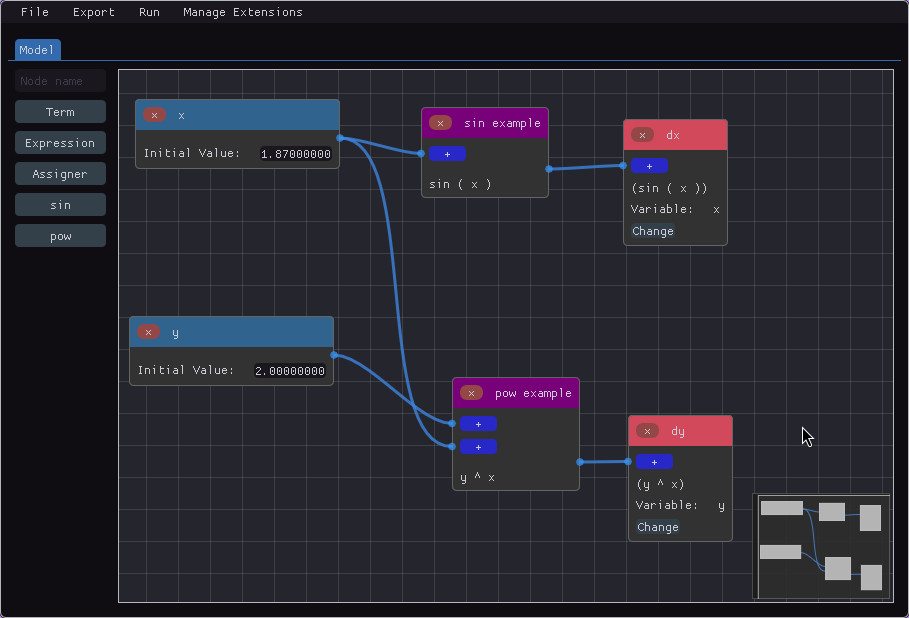
\includegraphics[width=\textwidth]{contents/imgs/ode-designer/ext-sin-pow.png}
            \end{figure}
        \end{column}
    \end{columns}
\end{frame}

\begin{frame}{Distribuição do Software}
    \begin{itemize}
        \item Como mencionado anteriormente, o software possui dependência do Python, assim como algumas bibliotecas da linguagem.
        \item Visto que o público-alvo do software não é necessariamente técnico, a maneira como seria distribuído o software se tornou um ponto chave.
        \item Portanto, foram desenvolvidas automações capazes de compilar e empacotar o software e todas as suas dependências.
        \begin{itemize}
            \item Para Linux, o uso de AppImages provê um arquivo único executável.
            \item Para Windows, SO que não possui uma ferramenta equivalente, uma pasta compactada é distribuída. A pasta contém o executável principal e as dependências necessárias.
        \end{itemize}
    \end{itemize}
\end{frame}
